\documentclass{article}
% --- watermark (auto-inserted) ---
\usepackage{xcolor}
\usepackage{xfp}% \fpeval; in the kernel since 2022, harmless on older LaTeX
\usepackage{draftwatermark}
\newlength{\watermarkTextWidth}
\AddToHook{begindocument/end}{%
  \SetWatermarkText{\normalfont Generated by The Agentic Scientist}%
  \SetWatermarkFontSize{10pt}%
  \SetWatermarkLightness{0.85}%
  \settowidth{\watermarkTextWidth}{\normalfont\fontsize{10pt}{12pt}\selectfont Generated by The Agentic Scientist}%
  \edef\watermarkScale{\fpeval{0.8 * sqrt(\paperwidth**2 + \paperheight**2) / \watermarkTextWidth}}%
  \edef\watermarkAngle{\fpeval{atand(\paperheight/\paperwidth)}}%
  \SetWatermarkScale{\watermarkScale}%
  \SetWatermarkAngle{\watermarkAngle}%
}
% --- end watermark ---
 % For LaTeX2e
\usepackage{paper,times}

\usepackage{hyperref}
\usepackage{url}
\usepackage{amsmath,amssymb}
\usepackage{graphicx}
\usepackage{booktabs}
\usepackage{subcaption}

\newcommand{\kver}{\hat{k}}

\title{How Many Comparisons Change the Leader? Refit-Verified Influence Perturbations of Bradley--Terry Leaderboards Across Evaluation Designs}
\iclrfinalcopy
\author{The Agentic Scientist}

\begin{document}
\maketitle

\begin{abstract}
Leaderboards for language models and sports rank participants by fitting a Bradley--Terry (BT) model to pairwise comparisons. It is rarely measured how much of the comparison data a reported ranking depends on. We measure the smallest perturbation we can find and certify that changes the leader or the top-$k$ set of a ridge BT leaderboard. A perturbation either drops comparisons or reverses their outcomes. The search orders comparisons by their first-order influence on the decisive score margin, and an exact refit verifies every reported size. We evaluate 15 cases spanning crowdsourced votes (Chatbot Arena), expert and GPT-4-judge annotations (MT-Bench), and two NBA seasons. In every design, tens of comparisons change the leader: 62 of 135,622 Arena votes (0.046\%), 92 expert and 143 GPT-4 judgments, and 7 and 16 NBA games. These sets are about $16\times$ smaller than random perturbations, and identical across seeds. The most fragile design depends on the scale and the target. As a fraction of the data Arena is the most fragile; by count, NBA is. Moving a top-$k$ boundary can cost one game, or more than changing the leader. All sizes are upper bounds; cross-design differences are descriptive, not causal.
% @evidence[[paper_data.json#final_evaluation.evaluation_evidence.episodes]]
% @evidence[[paper_data.json#final_evaluation.metrics.arena140k_top1_drop_frac]]
% @evidence[[paper_data.json#final_evaluation.metrics.mean_log2_ratio_vs_random]]
% @evidence[[analysis/derived_stats.json#n_rows_derived]]
\end{abstract}

\section{Introduction}
\label{sec:intro}

Pairwise-comparison leaderboards have become a central instrument of model evaluation. Chatbot Arena aggregates crowdsourced votes between two anonymous chatbots~\citep{Chiang2024ChatbotAA}. MT-Bench collects expert and GPT-4 judgments on a fixed question set~\citep{Zheng2023JudgingLW}. Sports ratings descend from the same paired-comparison tradition~\citep{Elo1978TheRO}. In each case a Bradley--Terry (BT) model~\citep{Bradley1952RankAO} turns the comparisons into scores, and the scores into a ranking. Rankings are then used to choose models, to advertise releases, and to compare research systems. Their confidence intervals usually come from resampling or asymptotic arguments~\citep{Efron1979BootstrapMA,Gao2021UncertaintyQI}. These describe \emph{random} variation, not how much \emph{specific} data the conclusion rests on. Recent work shows that crowdsourced leaderboards can be moved deliberately~\citep{Min2025ImprovingYM}, that evaluation practice shapes them~\citep{Singh2025TheLI}, and that dropping a small number of preferences can alter top Arena rankings~\citep{Huang2025DroppingJA}. What remains open is how this sensitivity \emph{compares across evaluation designs}, and how the answer depends on what is measured.

We ask: \emph{how small a verified perturbation of the comparison data changes the top-1 or the top-$k$ set of a ridge BT leaderboard? How does that size differ between crowdsourced votes, expert annotation, an LLM judge, and sports results?} We answer with a measurement instrument, not a new estimator. Following the drop-data robustness metric of \citet{Broderick2020AnAF}, we order comparisons by a one-step influence approximation~\citep{Cook2000DetectionOI,Koh2017UnderstandingBP} of their effect on the decisive score margin. We find the shortest prefix of that ordering whose removal (or outcome reversal) changes the target. An exact refit checks every candidate. Each reported size is therefore a certified \emph{upper bound} on the minimal perturbation, not an approximation.

Our central finding has two parts. First, in every design we study, tens of comparisons are enough to change the leader. The verified sets are about $16\times$ smaller than random perturbations of the same data (\S\ref{sec:res-validity}). Second, the question ``which design is most fragile?'' has no scale-free answer. Measured as a fraction of the data, the crowdsourced Arena leader is the most fragile (0.046\%) and the GPT-4-judge leader the least (5.96\%). Measured as a count, the NBA leaders are the most fragile (7 and 16 games). The target matters as much as the scale. In both NBA seasons, a single game changes the top-5 set. In MT-Bench, by contrast, the top-3 set costs more than the leader.
% @evidence[[analysis/derived_stats.json#cases]]
% @evidence[[paper_data.json#final_evaluation.metrics.mtbench_gpt4_top1_drop_frac]]

\paragraph{Contributions.}
(i) A measurement protocol for leaderboard fragility built on a refit-verified, influence-ordered perturbation finder; the finder is the provided baseline (starter) configuration, not a new algorithm of ours. The protocol covers two perturbation types (dropping and flipping comparisons) and two targets (top-1 and top-$k$ set). It is checked against a planted case with an enumerated minimum, a row-permutation control, and seed replay (\S\ref{sec:method}, \S\ref{sec:res-validity}).
(ii) A cross-design measurement on pinned public snapshots of four evaluation designs, with every size reported both as a count and as a fraction of the data (\S\ref{sec:res-main}).
(iii) Three regularities with stated limits. Flipping always needs fewer comparisons than dropping. The top-$k$ boundary can be far cheaper or dearer to move than the leader. Fragility rankings across designs reverse between the count and fraction scales (\S\ref{sec:res-contrasts}).
(iv) An explicit negative result: the search procedure we evaluate does not improve on the plain influence ordering. The pre-declared test of that improvement is unsupported, so we make no algorithmic-superiority claim (\S\ref{sec:res-validity}).

\begin{figure}[t]
\centering
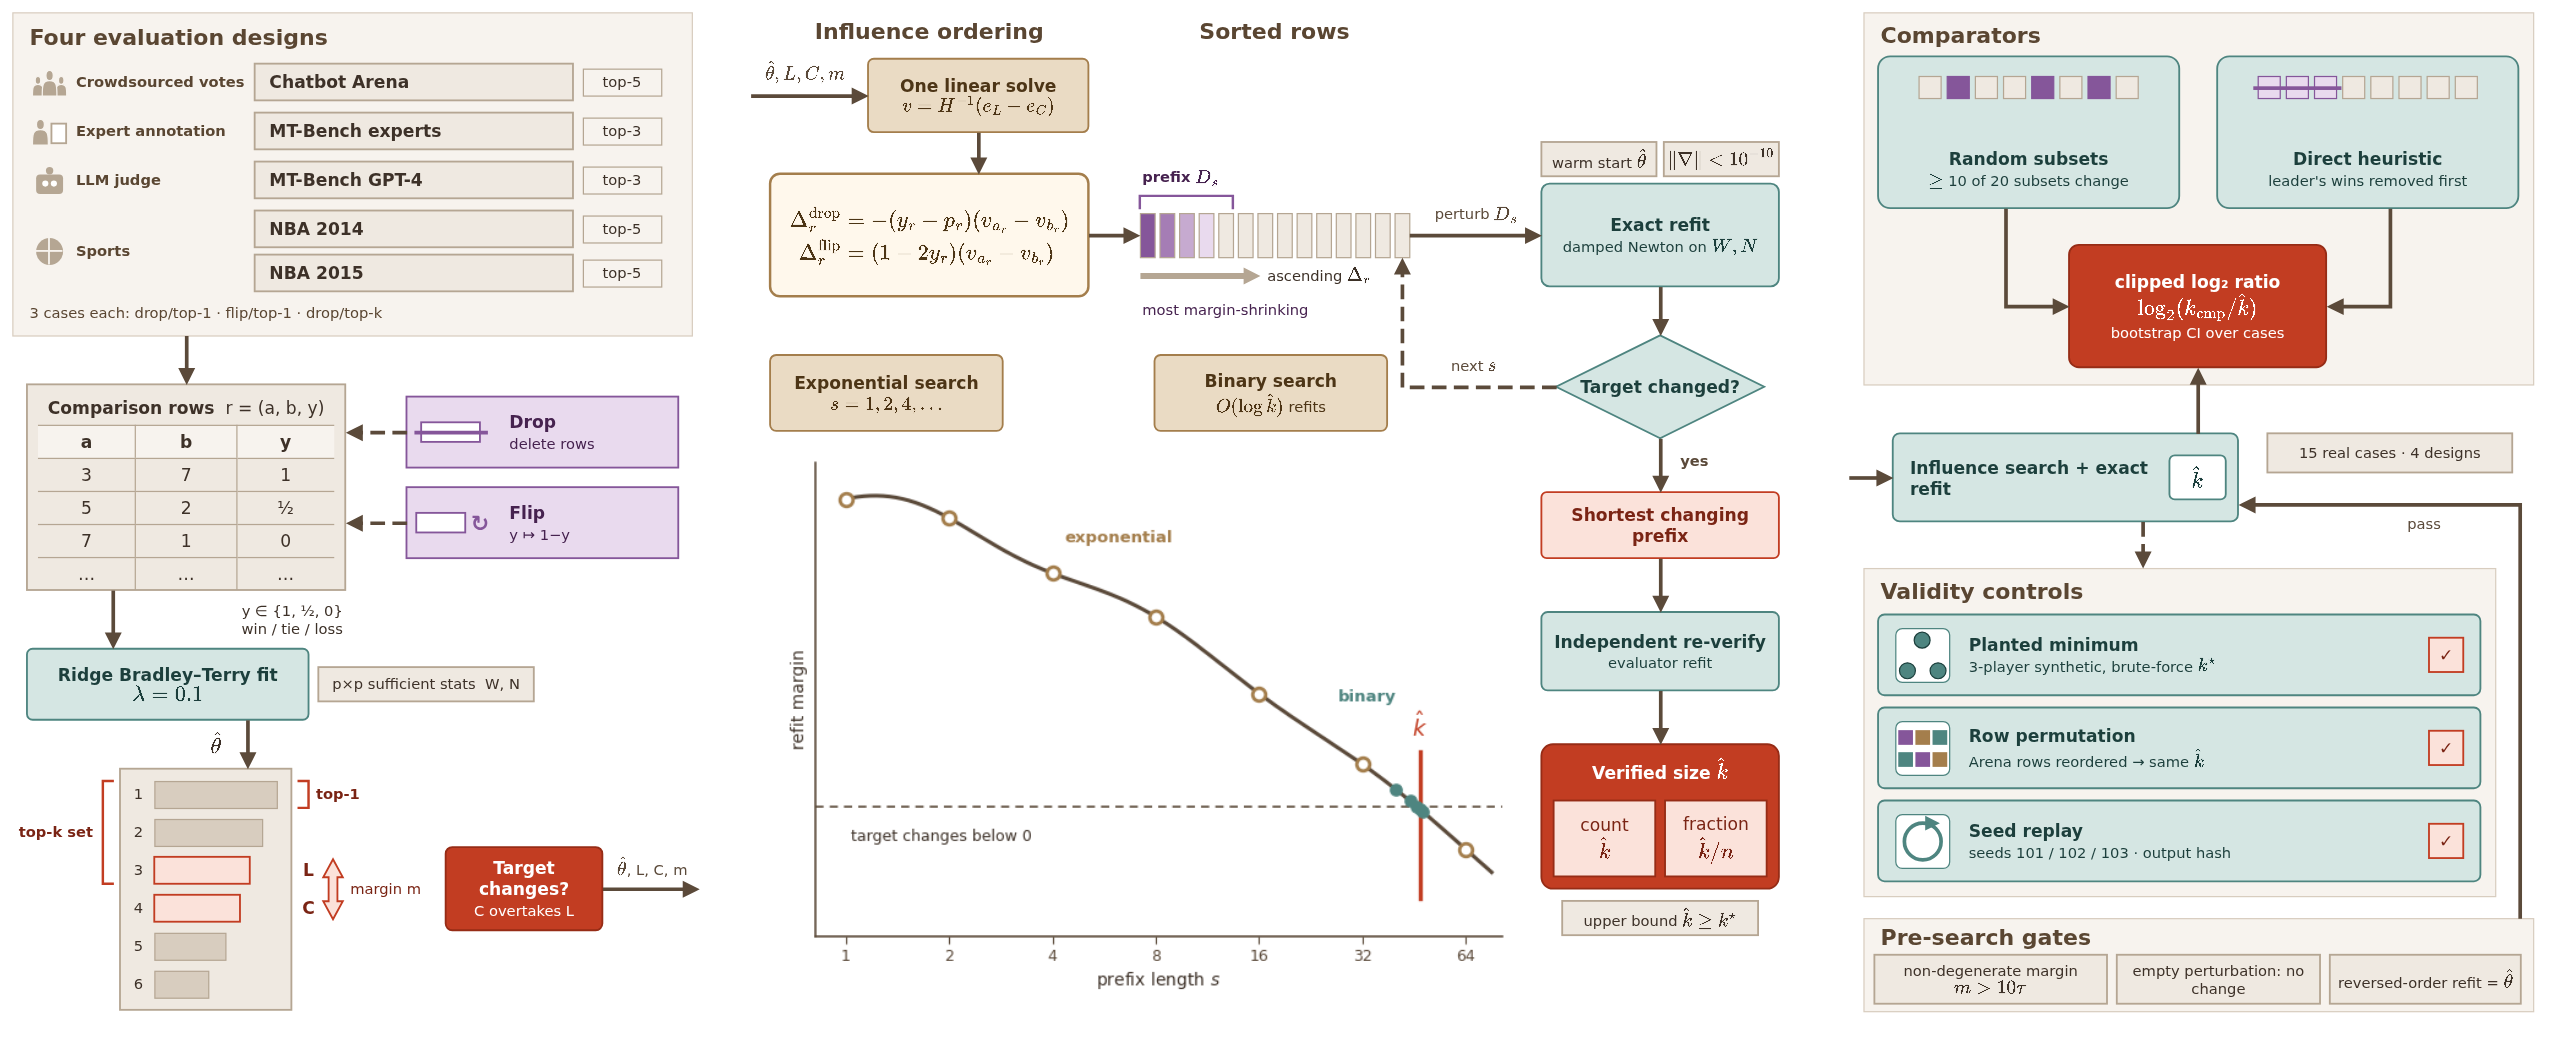
\includegraphics[width=0.95\textwidth]{figures/protocol_overview.png}
\caption{Protocol overview. Comparison rows from four evaluation designs are fit with a ridge Bradley--Terry model. Rows are ordered by their one-step influence on the decisive margin: leader vs.\ runner-up for top-1, or the $k$-th vs.\ $(k{+}1)$-th player for a top-$k$ set. The shortest prefix whose removal or outcome reversal changes the target is found by exponential and binary search. Every probe is an exact refit, and the final set is re-verified independently. Sizes are reported as a count $\kver$ and as a fraction $\kver/n$. A random-subset comparator, a direct leader--challenger heuristic, a planted-minimum control, a row-permutation control, and seed replay calibrate the instrument.}
\label{fig:overview}
\end{figure}

\section{Related Work}
\label{sec:related}

\paragraph{Paired-comparison models and ranking.}
The BT model~\citep{Bradley1952RankAO} and its extensions to ties~\citep{Davidson1970OnET} underlie most comparison leaderboards. Ties are often handled, as here, by counting them as half wins. Maximum-likelihood fitting is classical~\citep{Hunter2003MMAF}. Spectral and counting alternatives come with sample-complexity guarantees for recovering the top-$K$ items~\citep{Negahban2012RankCR,Chen2015SpectralMT,Chen2017SPECTRALMA,Shah2015SimpleRA}. Elo ratings play the same role in sports and games~\citep{Elo1978TheRO}. Uncertainty for BT scores is usually quantified by asymptotic theory~\citep{Gao2021UncertaintyQI} or the bootstrap~\citep{Efron1979BootstrapMA}, and the robustness of Elo-style rankings of language models has itself been examined~\citep{Boubdir2023EloUR}. These tools answer ``how variable is the ranking under resampling?''. We ask a worst-case, data-specific question: ``how few concrete comparisons does the ranking rest on?''.

\paragraph{Influence and drop-data robustness.}
Influence diagnostics go back to Cook's distance~\citep{Cook2000DetectionOI}. They were extended to nonlinear models~\citep{Monari2000WithdrawingAE} and to modern machine learning~\citep{Koh2017UnderstandingBP}, though they can be fragile for deep networks~\citep{Basu2020InfluenceFI}. Infinitesimal-jackknife approximations make leave-out analysis cheap~\citep{Giordano2018ASA}, and higher-order influence expansions refine it~\citep{Giordano2019AHS,Alaa2020DiscriminativeJQ}. \citet{Broderick2020AnAF} turn this machinery into a robustness metric, the approximate maximum influence perturbation: the smallest fraction of data whose removal can overturn a conclusion. For ordinary least squares in low dimensions, such drop-data conclusions can be audited with provable guarantees~\citep{Moitra2022ProvablyAO}. We adopt the drop-data question, apply it to rank conclusions of a BT fit, add an outcome-reversal perturbation, and certify every size by exact refits rather than reporting the linear approximation.

\paragraph{Manipulation and validity of LLM leaderboards.}
Chatbot Arena~\citep{Chiang2024ChatbotAA} and MT-Bench~\citep{Zheng2023JudgingLW} established crowdsourced and judge-based pairwise evaluation of chat models. Automatic judges have known biases, such as a preference for length, which can be partly corrected~\citep{Dubois2024LengthControlledAA}. \citet{Min2025ImprovingYM} show that a model's Arena ranking can be improved by rigging votes, and \citet{Singh2025TheLI} document how private testing and unequal data access distort the Arena leaderboard. \citet{Huang2025DroppingJA} report that dropping a handful of preferences can change top LLM rankings. Adversarial attacks on rank aggregation have also been analyzed as games between attacker and aggregator~\citep{Ma2022ATO}. On the estimation side, \citet{Patil2020RankAF} study ranking recovery under BTL-type models when an adversary corrupts a fraction of the pairwise comparisons, which is the setting our flip perturbation instantiates on fixed real data. We do not claim to be the first to show that an Arena leader is fragile. Our contribution is the controlled comparison across crowdsourced, expert, LLM-judge, and sports designs under one estimator and protocol. We also contrast drop and flip perturbations and top-1 and top-$k$ targets, and we show that cross-design conclusions depend on the size scale.

\section{Problem Setup}
\label{sec:setup}

\paragraph{Data and estimator.}
A case consists of $n$ comparison rows $r=(a_r,b_r,y_r)$ among $p$ players. The outcome is $y_r\in\{1,\tfrac12,0\}$: a win for $a_r$, a tie, or a win for $b_r$. The leaderboard is the ridge-penalized BT maximum-likelihood estimate
\begin{equation}
\hat\theta=\arg\max_{\theta\in\mathbb{R}^p}\;\sum_{r=1}^{n}\Big[y_r\log\sigma(\theta_{a_r}-\theta_{b_r})+(1-y_r)\log\sigma(\theta_{b_r}-\theta_{a_r})\Big]-\frac{\lambda}{2}\|\theta\|_2^2 ,
\label{eq:bt}
\end{equation}
where $\sigma$ is the logistic function and ties count as half a win for each side. The ridge weight $\lambda$ and the tolerance $\tau$ below are passed to the finder by the evaluation harness with each request; the harness specifies $\lambda=0.1$ and $\tau=10^{-6}$. The ridge term fixes the location of $\theta$ and keeps the fit finite even when the perturbation removes all of a player's losses. According to the harness's stated protocol, players with fewer than 50 comparisons are removed iteratively before fitting. The player set is then fixed: a player keeps its index even if every one of its rows is dropped. Equation~\eqref{eq:bt} depends on the data only through the $p\times p$ matrices of (half-)wins $W_{ij}$ and counts $N_{ij}$. A refit after any perturbation therefore costs $O(p^3)$ per Newton step, independent of $n$. The finder's refit implements exactly this objective (source locations in Appendix~\ref{app:repro}).

\paragraph{Targets.}
Let $S$ be the original top-$k$ set under $\hat\theta$. The \emph{top-$k$ target changes} after a perturbation if the refit $\tilde\theta$ satisfies $\max_{j\notin S}\tilde\theta_j>\min_{i\in S}\tilde\theta_i+\tau$. Top-1 is the special case $k=1$: some other player overtakes the leader. We study top-1 for every source, plus top-5 for Arena and NBA and top-3 for MT-Bench, which has few players.

\paragraph{Perturbations.}
A \emph{drop} perturbation deletes a set $D$ of rows. A \emph{flip} perturbation reverses the outcomes of a set $F$ of decided rows ($y\mapsto 1-y$). Ties cannot be flipped. Drops model missing or filtered data and targeted removal. Flips model mislabeled or adversarially cast votes: the data volume stays the same and only the verdicts change. The quantity of interest is the minimal size $k^\star$ of a set that changes the target. We report $\kver\ge k^\star$, the size of a set we construct and verify.

\paragraph{Two size scales.}
We report every size both as a count $\kver$ and as a fraction $\kver/n$, and we argue that neither alone is adequate. The fraction is the natural robustness scale of \citet{Broderick2020AnAF}. It answers ``what share of the evidence must be wrong?'', which is the relevant question for random noise and data-quality concerns. The count answers ``how many comparisons must an adversary control?'', which is the relevant question for manipulation, where cost scales with votes, not with shares. The two scales can order designs differently when $n$ varies by two orders of magnitude, as it does here. We treat that disagreement as a finding, not a nuisance (\S\ref{sec:res-contrasts}).

\paragraph{What is inspectable.}
The study has two components. The \emph{finder}, which constructs perturbation sets, is released in full, and every statement we make about it can be checked against its source. The \emph{evaluation harness}, which builds the cases, re-verifies each returned set with its own refit, runs the comparators and controls, and computes all reported scores and fractions, is not part of the artifacts accompanying this paper. Its numerical outputs are our evidence. Its internal settings (the player filter, tie mapping, comparator and control construction, data splitting, and scoring rules) are described below as the harness's \emph{stated protocol}. They could not be checked against source here.

\section{Method: Refit-Verified Influence Ordering}
\label{sec:method}

\paragraph{Influence of one row on the decisive margin.}
Let $L$ and $C$ be the $k$-th and $(k{+}1)$-th players under $\hat\theta$; for top-1 these are the leader and the runner-up. Let $m=\hat\theta_L-\hat\theta_C>0$ be the decisive margin and $c=e_L-e_C$. The negative Hessian of \eqref{eq:bt} at $\hat\theta$ is $H=\sum_r p_r(1-p_r)(e_{a_r}-e_{b_r})(e_{a_r}-e_{b_r})^\top+\lambda I$, with $p_r=\sigma(\hat\theta_{a_r}-\hat\theta_{b_r})$. Row $r$ contributes the gradient $(y_r-p_r)(e_{a_r}-e_{b_r})$. Removing it moves the optimum by approximately $-H^{-1}(y_r-p_r)(e_{a_r}-e_{b_r})$~\citep{Cook2000DetectionOI,Koh2017UnderstandingBP}. With $v=H^{-1}c$, the first-order effects of dropping or flipping row $r$ on the margin are therefore
\begin{equation}
\Delta^{\text{drop}}_r=-(y_r-p_r)(v_{a_r}-v_{b_r}),\qquad
\Delta^{\text{flip}}_r=(1-2y_r)(v_{a_r}-v_{b_r}).
\label{eq:influence}
\end{equation}
Rows are sorted by ascending $\Delta_r$, so the rows that shrink the margin most come first. One linear solve gives $v$; the ordering costs $O(p^3+n\log n)$. Equation~\eqref{eq:influence} also suggests two qualitative regularities. First, for a row won by $a_r$ ($y_r=1$), the flip effect exceeds the drop effect by the factor $1/(1-p_r)\ge 1$, which equals 2 for an even match-up. Flips should therefore need fewer rows; we compare this with the verified sizes in \S\ref{sec:res-contrasts}. Second, $|v_{a}-v_{b}|$ shrinks as the information about the $L$--$C$ contrast grows. This suggests that the \emph{count} needed scales with the margin times that information, while the \emph{fraction} also falls when the rows touching $L$ and $C$ are a small share of a large data set. We did not measure decisive margins, boundary gaps, or the share of rows involving the decisive pair, so this second regularity is a hypothesis that our data cannot test.

\paragraph{Exact verification by prefix search.}
The linear approximation only orders rows; it never sets the reported size. For a prefix $D_s$ of length $s$ we refit \eqref{eq:bt} exactly. The refit is a damped Newton method on the perturbed sufficient statistics, warm-started at $\hat\theta$ and stopped once the largest absolute gradient entry falls below $10^{-10}$, and the target condition is tested on the result. The search doubles $s=1,2,4,\dots$ until a prefix changes the target, then bisects between the last failing and the first succeeding length. This requires $O(\log \kver)$ refits. The search returns the shortest changing prefix it locates, and the harness re-verifies the returned set with its own independent refit. Because the refit after a perturbation is not guaranteed to be monotone in $s$, bisection may miss a shorter changing prefix. Even then, the returned set is a valid certificate. The finder is a single NumPy module (Appendix~\ref{app:repro}). It is deterministic: its seed only initializes a random generator that the search never uses.

\paragraph{What a verified size means.}
$\kver$ is an \emph{upper bound} on $k^\star$: an explicit set of $\kver$ rows exists whose perturbation changes the target under the exact estimator. Nothing smaller is ruled out. Computing $k^\star$ is a combinatorial search problem. Provable auditing is known only in special settings such as low-dimensional least squares~\citep{Moitra2022ProvablyAO}. Even there, exact search and certificates that no smaller set exists become computationally demanding beyond a few dimensions, while greedy and influence-based heuristics only exhibit sets and therefore give upper bounds~\citep{Freund2023TowardsPR}. We do not claim to solve the problem on real data. Instead, we check the instrument on a planted case whose minimum the harness computes by enumeration (below).

\paragraph{Comparators.}
The harness runs two comparators on identical data. We describe them according to its stated protocol. \emph{Random:} the smallest $s$ such that at least 10 of 20 uniformly random size-$s$ subsets change the target. The search uses the same doubling and bisection and is capped at half the rows. This is a noise reference: the size at which a \emph{typical} perturbation, not a chosen one, flips the conclusion. \emph{Direct heuristic:} the ``obvious attack''. It first removes the leader's wins over the challenger, then the leader's other wins in order of decreasing opponent strength. We summarize each comparator per case as $\mathrm{clip}(\log_2(k_{\text{cmp}}/\kver),-4,4)$, average it over seeds, then over the 15 real cases. The harness reports a 95\% percentile-bootstrap interval over cases (stated as 2{,}000 resamples).

\paragraph{Validity controls.}
These are also part of the harness's stated protocol. \emph{Planted minimum:} a synthetic three-player case with a near-tied leader pair. The harness computes its exact minimal drop size by brute-force enumeration over per-pair winner counts, which are sufficient statistics for \eqref{eq:bt}. \emph{Row permutation:} the Arena drop/top-1 case with its rows presented in a different order. A correct instrument must return the same size. \emph{Seed replay:} each case runs under three seeds, and one episode is replayed and its output hash compared. Before any search, the harness is stated to check each case. It rejects cases with a degenerate decisive margin ($m\le 10\tau$). It also requires that the empty perturbation leaves the target unchanged and that a refit on reversed row order reproduces $\hat\theta$.

\paragraph{Data and protocol.}
Table~\ref{tab:cases} lists the cases. The four designs are crowdsourced votes from the Chatbot Arena 140k human-preference release~\citep{Chiang2024ChatbotAA}; expert human and GPT-4 pairwise judgments of MT-Bench answers~\citep{Zheng2023JudgingLW}; and NBA games from two seasons of the FiveThirtyEight Elo record, the 2014 and 2015 seasons in that file's labeling, with each game a comparison between two teams, following the long use of BT models for sports tournaments~\citep{Cattelan2013DynamicBM}. We fit a static BT model to each season, without the time-varying strengths such models can include. Under the harness's stated protocol, Arena ``tie'' and ``both bad'' votes and MT-Bench tie judgments become ties ($y=\tfrac12$); NBA games have no ties. Each design contributes three cases: drop/top-1, flip/top-1, and drop/top-$k$. With the two controls this gives 17 cases. Method choices were made on separate development data, stated by the harness to be the Arena 55k release and the NBA 1983 season. The harness is also stated to exclude final rows whose content hash appears in the development data. Neither the split nor its overlap can be inspected in our artifacts. The 17 cases were then run once in a sealed evaluation under seeds 101, 102, and 103. Every episode either returns a set that the harness verifies, or counts as a failure; none failed. The sealed evaluation completed with a qualified outcome, and the replayed episode matched. The record gives this overall outcome only, without per-gate diagnostics.
% @evidence[[paper_data.json#final_evaluation.metrics.failed_episode_fraction]]
% @evidence[[paper_data.json#final_evaluation.outcome]]

\begin{table}[t]
\centering
\caption{Evaluation designs and cases. $n$ is the number of comparison rows after filtering, recovered exactly from the evaluator's reported fraction $\kver/n$ and the verified size $\kver$ (Appendix~\ref{app:derivation}). Every source contributes drop/top-1, flip/top-1, and drop/top-$k$ cases.}
\label{tab:cases}
\small
\begin{tabular}{@{}llrcl@{}}
\toprule
Design & Source (pinned snapshot) & $n$ & top-$k$ & What a row is \\
\midrule
Crowdsourced votes & Chatbot Arena human pref.\ (140k) & 135{,}622 & 5 & one user vote \\
Expert annotation & MT-Bench human judgments & 3{,}355 & 3 & one expert judgment \\
LLM judge & MT-Bench GPT-4 pair judgments & 2{,}400 & 3 & one GPT-4 verdict \\
Sports & NBA, 2014 season (FiveThirtyEight) & 1{,}319 & 5 & one game \\
Sports & NBA, 2015 season (FiveThirtyEight) & 1{,}311 & 5 & one game \\
\midrule
Control & planted 3-player case (synthetic) & -- & -- & drop/top-1 only \\
Control & Arena drop/top-1 with rows permuted & 135{,}622 & -- & drop/top-1 only \\
\bottomrule
\end{tabular}
% @evidence[[analysis/derived_stats.json#n_rows_derived]]
\end{table}

\section{Results}
\label{sec:results}

\subsection{The instrument matches a planted minimum, is order-invariant, and is deterministic}
\label{sec:res-validity}

Table~\ref{tab:validity} collects the evidence that the measured sizes mean what we claim. On the planted synthetic case, the verified drop size is 8 and the control score is 0. The harness defines this score as $\min(0,\log_2(k^\star/\kver))$ with $k^\star$ its enumerated minimum. Under that stated definition, a value of 0 means the instrument returned the brute-force minimum, so here, at least, the upper bound is tight. Under row permutation, the Arena drop/top-1 size is 62 in both presentations (control score 0), so the result does not depend on row order. All 15 real-case sizes are identical across seeds 101, 102, and 103. The replayed episode reproduced its output hash (replay match 1.0), and no episode failed. Since the finder is deterministic, seed agreement shows reproducibility. It does \emph{not} measure sampling uncertainty (\S\ref{sec:limitations}).
% @evidence[[paper_data.json#final_evaluation.metrics.synthetic_control_score]]
% @evidence[[paper_data.json#final_evaluation.metrics.permutation_control_score]]
% @evidence[[paper_data.json#final_evaluation.metrics.replay_match]]

Against the random comparator, the influence-ordered sets are far smaller. The mean clipped $\log_2(k_{\text{rand}}/\kver)$ is 3.975, with 95\% CI [3.934, 4.0]. This corresponds to a geometric-mean factor of about $15.7\times$. The upper end of the interval sits at the clip value of 4, so most cases are censored, and the true advantage is \emph{at least} this large. Fragility to chosen perturbations is therefore a different quantity from fragility to noise. A leader that survives typical random corruption of tens of comparisons can still fall to a targeted set of the same size.
% @evidence[[paper_data.json#final_evaluation.metrics.mean_log2_ratio_vs_random]]
% @evidence[[analysis/derived_stats.json#random_ratio_x]]

The direct heuristic is visible only through family scores, which are 0 for the Arena, GPT-4-judge, and NBA families and $-0.0053$ for MT-Bench experts. Under the harness's stated scoring rule (Appendix~\ref{app:details}), a score of 0 means the heuristic was never smaller than the influence ordering in that family, and the negative MT-Bench-expert score means it was marginally smaller in at least one case. Because the scoring rule is stated rather than inspectable, and per-case heuristic sizes are not recorded, we read this only as weak evidence that the ordering matches or beats the obvious ``remove the leader's wins'' attack in most cases, but not uniformly.
% @evidence[[paper_data.json#final_evaluation.metrics.mtbench_human_score]]

\paragraph{No improvement over the plain influence ordering.}
The configuration evaluated here \emph{is} the influence ordering plus verified prefix search. Its sizes coincide with those of the harness's own one-step-influence comparator: the mean $\log_2$ ratio is 0.0, with CI [0.0, 0.0], and the four reported top-1 drop fractions are equal to the reported precision. The pre-declared test of a strict improvement over this ordering (CI lower bound $>0$) is therefore \emph{not supported}. We make no claim of algorithmic superiority. Three refined search configurations were designed but none was scored; the cause is not recorded in the evaluation evidence. Their effect is unknown, not negative (Appendix~\ref{app:negative}).
% @evidence[[paper_data.json#final_evaluation.metrics.claim_supported]]
% @evidence[[paper_data.json#final_evaluation.metrics.mean_log2_ratio_vs_amip]]
% @evidence[[paper_data.json#downstream_study.attempt_counts]]

\begin{table}[t]
\centering
\caption{Instrument validation and comparators (sealed evaluation, three seeds). Ratios are mean over the 15 real cases of $\mathrm{clip}(\log_2(k_{\text{cmp}}/\kver),-4,4)$ with a 95\% bootstrap CI over cases. Positive values mean the comparator needed more rows. $^\dagger$Interpretation relies on the harness's stated scoring rule.}
\label{tab:validity}
\footnotesize
\begin{tabular}{@{}lll@{}}
\toprule
Check & Result & Interpretation \\
\midrule
Planted minimum (synthetic) & $\kver=8$; score $0$ & equals brute-force minimum \\
Row permutation (Arena) & $\kver=62$ vs.\ $62$; score $0$ & invariant to row order \\
Seed agreement (101/102/103) & 15/15 real cases identical & deterministic \\
Replay of one episode & match $=1.0$ & identical output hash \\
Failed episodes & fraction $0.0$ & every proposal verified \\
\midrule
vs.\ random subsets & $3.975$ [$3.934$, $4.0$] & $\approx 15.7\times$ fewer rows \\
vs.\ one-step influence ordering & $0.0$ [$0.0$, $0.0$] & identical; no superiority \\
vs.\ direct heuristic (family scores) & Arena $0$, MTB-GPT-4 $0$, NBA $0$ & never worse$^\dagger$ \\
 & MTB-expert $-0.0053$ & heuristic smaller in $\ge$1 case$^\dagger$ \\
\bottomrule
\end{tabular}
% @evidence[[paper_data.json#final_evaluation.metrics]]
% @evidence[[analysis/derived_stats.json#controls]]
\end{table}

\subsection{Tens of comparisons change the leader in every design}
\label{sec:res-main}

\begin{figure}[t]
\centering
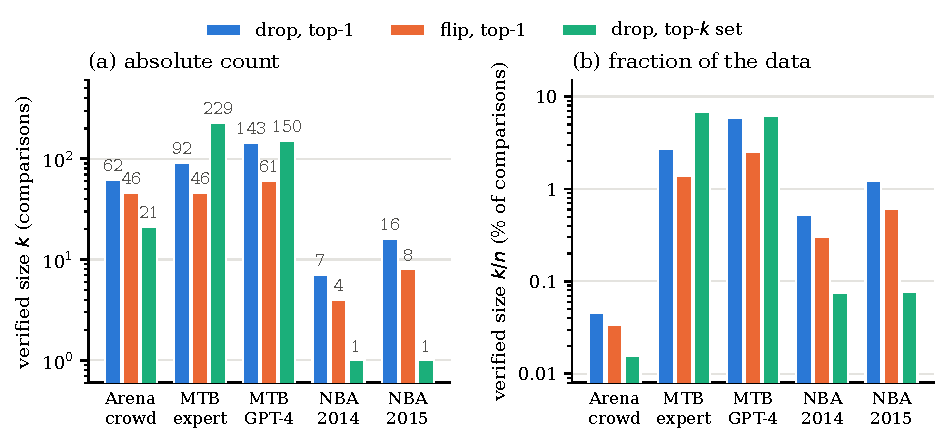
\includegraphics[width=\textwidth]{figures/fragility_by_design_two_scales.pdf}
\caption{Verified perturbation sizes for all 15 real cases, on two scales (log axes). (a) Count $\kver$ of comparisons dropped or flipped; integers are annotated. (b) The same sizes as a percentage of the source's comparisons, $\kver/n$. Colors mark the target and perturbation; top-$k$ is top-5 for Arena and NBA and top-3 for MT-Bench (MTB). Sizes are identical across the three seeds.}
\label{fig:main}
\end{figure}

Figure~\ref{fig:main} shows the main result. The leader changes after dropping 62 Arena votes, 92 expert judgments, 143 GPT-4 judgments, 7 games of the 2014 NBA season, or 16 games of the 2015 season. Flipping requires 46, 46, 61, 4, and 8 rows, respectively. As fractions, the drop sizes are 0.046\% of Arena, 2.74\% of MT-Bench expert judgments, 5.96\% of GPT-4 judgments, and 0.53\% and 1.22\% of the two NBA seasons. The NBA fractions average 0.876\%.
% @evidence[[analysis/derived_stats.json#cases]]
% @evidence[[paper_data.json#final_evaluation.metrics.nba_top1_drop_frac]]
% @evidence[[paper_data.json#final_evaluation.metrics.mtbench_human_top1_drop_frac]]

Two readings follow. First, \emph{no design is robust in absolute terms.} The largest top-1 set we needed is 143 comparisons, and the smallest is 4 flipped games. These are upper bounds: sets of this size provably exist, and smaller ones may. Second, \emph{the 135,622-vote Arena leader is not protected by its data volume.} Its 62-vote certificate is a smaller share of the data than any other leader's by more than an order of magnitude. One explanation consistent with Eq.~\eqref{eq:influence} is that a large data set gives precision for the average contrast but not for the specific contrast at the top, if only a small share of rows involves the leader and runner-up. We did not measure that share or the decisive margin, so this explanation is a hypothesis, not a finding.
% @evidence[[paper_data.json#final_evaluation.metrics.arena140k_top1_drop_frac]]

\subsection{Drop vs.\ flip, top-1 vs.\ top-$k$, and the scale reversal}
\label{sec:res-contrasts}

\paragraph{Flipping is always cheaper than dropping.}
In all five sources, the verified flip size for top-1 is smaller than the drop size. The ratio of drop to flip size is 1.35 for Arena, 2.0 for MT-Bench experts, 2.34 for the GPT-4 judge, 1.75 for NBA 2014, and 2.0 for NBA 2015. This matches the first-order prediction of Eq.~\eqref{eq:influence}. Reversing a verdict both removes evidence for the leader and adds evidence against it, so its effect exceeds that of a drop by the factor $1/(1-p_r)$, which is near 2 for close match-ups. Arena's ratio, the furthest from 2, is not explained by our data. Ties can be dropped but not flipped, and the approximation ignores refitting, so we do not over-interpret it. For manipulation threat models, the flip size is the relevant one: an actor who controls a vote controls its direction.
% @evidence[[analysis/derived_stats.json#drop_over_flip_top1]]

\paragraph{The top-$k$ boundary can be far cheaper, or dearer, than the leader.}
Moving the top-5 set needs 21 Arena votes, against 62 for the leader. In \emph{both} NBA seasons, a single game suffices. In MT-Bench the top-3 set costs more than the leader: 229 vs.\ 92 expert judgments and 150 vs.\ 143 GPT-4 judgments. A natural hypothesis, again from Eq.~\eqref{eq:influence}, is that the cost depends on the score gap and information at the boundary being tested rather than on the leader's lead; for example, the NBA 5th and 6th teams may be nearly tied. We did not record boundary gaps, so we cannot confirm this. The harness's stated degenerate-margin check excludes only near-exact ties ($m\le 10\tau$). Either way, ``is the top-$k$ stable?'' and ``is the leader stable?'' are different questions, and a leaderboard can pass one and fail the other.
% @evidence[[analysis/derived_stats.json#topk_over_top1_drop]]

\begin{figure}[t]
\centering
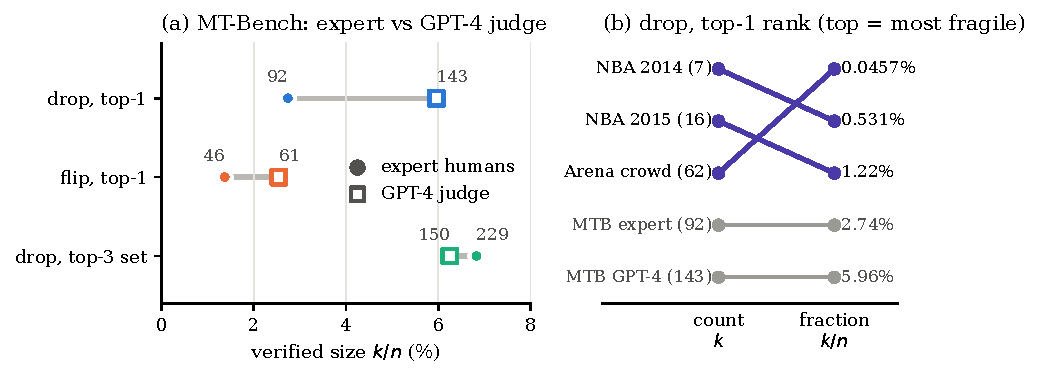
\includegraphics[width=\textwidth]{figures/controlled_contrasts.pdf}
\caption{Controlled contrasts. (a) MT-Bench: the same question set judged by expert humans (filled circles) and by GPT-4 (open squares). Values are $\kver/n$ in percent, with counts annotated. The GPT-4 leader needs a larger share of its data to change for top-1, but a smaller one for the top-3 set. (b) Fragility rank of the drop/top-1 cases by count (left, with $\kver$) and by fraction (right, with $\kver/n$). Rank 1 (top) is the most fragile. The ordering of Arena and the NBA seasons reverses between scales (purple).}
\label{fig:contrasts}
\end{figure}

\paragraph{Expert humans vs.\ an LLM judge on the same questions.}
MT-Bench is the closest thing to a controlled comparison in our data: the same benchmark is judged by experts and by GPT-4 (Fig.~\ref{fig:contrasts}a). For top-1, the GPT-4-judge leader is harder to dislodge, at 143 vs.\ 92 drops (5.96\% vs.\ 2.74\%) and 61 vs.\ 46 flips. For the top-3 set the order reverses: 150 vs.\ 229 drops (6.25\% vs.\ 6.83\%). Neither annotation source is uniformly more robust. The two sources also differ in $n$ (2,400 vs.\ 3,355), in tie rates, and possibly in which model leads, since player identities are hidden from the finder. The contrast is therefore not a causal estimate of a ``judge effect''.
% @evidence[[analysis/derived_stats.json#cases]]
% @evidence[[paper_data.json#final_evaluation.metrics.mtbench_gpt4_top1_flip_frac]]

\paragraph{Fragility rankings reverse between scales.}
Figure~\ref{fig:contrasts}b orders the five drop/top-1 cases by count and by fraction. By count, the two NBA seasons are the most fragile (7, 16), followed by Arena (62). By fraction, Arena moves to first place (0.0457\%), ahead of NBA 2014 (0.531\%) and NBA 2015 (1.22\%). The two MT-Bench sources stay last on both scales. A cross-benchmark statement such as ``crowdsourced leaderboards are more fragile than sports tables'' is therefore true on one natural scale and false on the other. Any such comparison must name its scale and justify it by the threat model (\S\ref{sec:setup}).
% @evidence[[analysis/derived_stats.json#cases]]

\section{Discussion and Limitations}
\label{sec:limitations}

\paragraph{What the evidence supports.}
For one fixed and widely used estimator, the following holds across four evaluation designs. Explicit, verified sets of tens of comparisons change the leader. Typical random perturbations need roughly 16 times as many rows. The relative fragility of designs depends on whether size is counted or proportioned, and on whether the conclusion is about the leader or a top-$k$ set. The protocol appears cheap. The recorded episode time per seed, over all 17 cases including the 135,622-row Arena case, was about 16\,s (15.5--16.3\,s). The record does not state what this time includes, and we did not profile it; a plausible but unmeasured reason for the low cost is that each refit acts on $p\times p$ sufficient statistics. For practitioners, this suggests reporting a verified drop and flip size alongside resampling intervals, for both the leader and any advertised top-$k$ claim.
% @evidence[[analysis/derived_stats.json#episode_durations_seconds]]

\paragraph{Upper bounds, not minima.}
Every size is an upper bound $\kver\ge k^\star$. Exactness is demonstrated only on the three-player planted case. On real data the true minimum may be smaller, possibly by a lot for cases with many players. Certifying lower bounds is hard even for least squares in a few dimensions~\citep{Moitra2022ProvablyAO,Freund2023TowardsPR}, and a BT fit with tens of players is well outside that regime. Statements such as ``the leader rests on 62 votes'' should be read as ``at most 62 votes''.

\paragraph{No sampling uncertainty on $\kver$.}
The three seeds give identical sizes because the finder is deterministic. They do not quantify how $\kver$ would vary under resampling of comparisons or under a different data snapshot. The bootstrap intervals in Table~\ref{tab:validity} are over cases, for comparator ratios, not over data. The random-comparator summary is censored at the clip of $\log_2=4$.

\paragraph{One estimator, one snapshot per source.}
All results use ridge BT with ties counted as half wins and, per the harness specification, $\lambda=0.1$ and a 50-comparison minimum per player. Other choices could change sizes, sometimes qualitatively. Examples include Elo-style online updates~\citep{Boubdir2023EloUR}, a Davidson tie model~\citep{Davidson1970OnET}, a different penalty, or style-controlled scores. Each design is represented by a single snapshot, and sports by two seasons. We have no within-design replication across releases.

\paragraph{Confounded cross-design differences.}
The designs differ in $n$, number of players, comparison-graph structure, tie rate, and the size of the decisive margin. With one case per design and target, we cannot attribute differences to the design itself, such as crowd versus judge. The cross-design statements are descriptive.

\paragraph{Comparator and search coverage.}
The direct heuristic is reported only at family level, so per-case heuristic sizes are unknown. More generally, comparator, control, and scoring details come from the harness's stated protocol, whose source is not among our artifacts. We evaluated one search configuration, the influence ordering with verified prefix search. Three refined variants were designed but not scored, so whether they find materially smaller sets remains open. Our sizes are thus conservative descriptions of fragility, not tight ones.

\section{Conclusion}
\label{sec:conclusion}

We measured how many comparisons must be dropped or reversed to change a Bradley--Terry leaderboard. The instrument orders comparisons by their influence on the decisive margin and certifies each size by exact refits; on a planted case it matches the minimum the evaluation harness computes by enumeration. Across crowdsourced votes, expert and LLM-judge annotations, and professional sports, tens of comparisons suffice to change the leader. These sets are roughly sixteen times smaller than random perturbations: fragility to chosen data differs from fragility to noise. Cross-design comparisons are scale- and target-dependent. The Arena leader is the most fragile as a share of its data but not as a count. NBA top-5 sets move with one game. MT-Bench top-3 sets resist more than their leaders. Expert and GPT-4 judges trade places between targets. We therefore recommend reporting verified fragility on both scales and for each advertised target. Such reports should be read as upper bounds on a fixed estimator, not as minima or causal properties of an evaluation design. Tighter certificates, data-resampling uncertainty for $\kver$, and controlled within-design replications are the natural next steps.

% IMPORTANT: \clearpage flushes all pending floats before references so that
% body-page counting excludes reference-only pages.  Do NOT remove.
\clearpage
\bibliography{references}
\bibliographystyle{paper}

\clearpage
\appendix
\section{Supplementary Information}
\label{app:si}

\subsection{Per-case verified sizes}
\label{app:percase}

Table~\ref{tab:percase} lists every case of the sealed evaluation. Each size is the same under seeds 101, 102, and 103. The recorded episode time per seed, summed over all 17 cases, was 15.99\,s, 15.55\,s, and 16.33\,s. The evaluation record gives one duration per seed and does not specify which steps it covers.
% @evidence[[paper_data.json#final_evaluation.evaluation_evidence.episodes]]
% @evidence[[analysis/derived_stats.json#episode_durations_seconds]]

\begin{table}[h]
\centering
\caption{Verified sizes per case (identical for seeds 101/102/103). $n$ is derived as in Appendix~\ref{app:derivation}. Percentages are $100\,\kver/n$.}
\label{tab:percase}
\small
\begin{tabular}{@{}llrrr@{}}
\toprule
Source & Case & $\kver$ & $n$ & $\kver/n$ (\%) \\
\midrule
Arena (crowd) & drop, top-1 & 62 & 135{,}622 & 0.0457 \\
 & flip, top-1 & 46 & 135{,}622 & 0.0339 \\
 & drop, top-5 set & 21 & 135{,}622 & 0.0155 \\
MT-Bench (expert) & drop, top-1 & 92 & 3{,}355 & 2.74 \\
 & flip, top-1 & 46 & 3{,}355 & 1.37 \\
 & drop, top-3 set & 229 & 3{,}355 & 6.83 \\
MT-Bench (GPT-4 judge) & drop, top-1 & 143 & 2{,}400 & 5.96 \\
 & flip, top-1 & 61 & 2{,}400 & 2.54 \\
 & drop, top-3 set & 150 & 2{,}400 & 6.25 \\
NBA 2014 & drop, top-1 & 7 & 1{,}319 & 0.531 \\
 & flip, top-1 & 4 & 1{,}319 & 0.303 \\
 & drop, top-5 set & 1 & 1{,}319 & 0.0758 \\
NBA 2015 & drop, top-1 & 16 & 1{,}311 & 1.22 \\
 & flip, top-1 & 8 & 1{,}311 & 0.610 \\
 & drop, top-5 set & 1 & 1{,}311 & 0.0763 \\
\midrule
Synthetic control & drop, top-1 & 8 & -- & -- \\
Permutation control (Arena) & drop, top-1 & 62 & 135{,}622 & 0.0457 \\
\bottomrule
\end{tabular}
% @evidence[[analysis/derived_stats.json#cases]]
\end{table}

\subsection{Recovering $n$ from the evaluation record}
\label{app:derivation}

The evaluation record reports, for each family, the top-1 drop and flip fractions $\kver/n$, averaged over seeds and, for NBA, over the two seasons. For Arena and the two MT-Bench sources, $n=\kver_{\text{drop}}/(\kver/n)_{\text{drop}}$; this yields 135,622, 3,355, and 2,400 to within floating-point error. For NBA, the season-mean drop fraction $\tfrac12(7/n_{14}+16/n_{15})=0.8756\%$ and flip fraction $\tfrac12(4/n_{14}+8/n_{15})=0.4567\%$ form a $2\times2$ linear system in $(1/n_{14},1/n_{15})$. Its solution gives $n_{14}=1{,}319$ and $n_{15}=1{,}311$. The two seasons sum to 2,630 games; we could not check this against the harness's season file, which is not among our artifacts. The script \nolinkurl{analysis/derive_stats.py} performs this derivation from \texttt{paper\_data.json} and writes \nolinkurl{analysis/derived_stats.json}.
% @evidence[[analysis/derive_stats.py]]
% @evidence[[paper_data.json#final_evaluation.metrics.nba_top1_flip_frac]]

\subsection{Estimator, cases, comparators and controls in detail}
\label{app:details}

This subsection records the evaluation harness's stated protocol. The harness source is not among the artifacts accompanying this paper, so these details are reported as specified and could not be inspected. Only the statements about what the finder receives are confirmed by the finder's own interface documentation (\nolinkurl{source_evidence/downstream/program/src/program.py}, lines 1--46).

\paragraph{Case construction.}
For each real source, the harness is stated to load the pinned resource, drop rows shared with the development split, shuffle the rows with a fixed private seed, and iteratively remove players with fewer than 50 comparisons. Players are relabelled per case, so the finder receives only integer identifiers and outcomes, never names, text, labels, or dates (confirmed by the interface documentation). The original top-$k$ set, the decisive pair, and the margin come from the harness's own fit.

\paragraph{Random comparator.}
For a candidate size $s$, 20 uniformly random subsets of size $s$ are drawn from the perturbable rows, with early stopping. The size counts as changing the target if at least 10 of them change it. The smallest such $s$ is found by doubling and bisection up to half of the perturbable rows. Failure to find one is recorded as $n+1$ (censored). Each case and size uses its own fixed random stream.

\paragraph{Direct heuristic.}
Rows where the leader beat the challenger come first, in index order. Then come the leader's other wins, sorted by decreasing fitted strength of the beaten opponent. The same verified prefix search is applied.

\paragraph{Planted control.}
Three players meet in three pairs of 50--80 games each. One pair is nearly balanced, with one to three wins above an even split; the other pairs have win rates between 0.55 and 0.70. Before the case is accepted, its exact minimal drop size is found by enumerating all compositions of per-pair winner classes up to size 8. Cases with an exact minimum below 2 are rejected. The finder returned a size-8 set, and the control score of 0 indicates equality with the enumerated minimum under the stated score definition.

\paragraph{Scoring.}
For real cases, each seed's score is $\mathrm{clip}(\log_2(\min(k_{\text{infl}},k_{\text{heur}})/\kver),-4,4)$. Here $k_{\text{infl}}$ is the evaluator's one-step-influence comparator, and an unverified proposal scores $-4$. Family scores are weighted means over the family's cases. If the scoring rule is as stated, then, because the evaluated finder reproduces $k_{\text{infl}}$ (mean log-ratio 0.0, CI [0.0, 0.0]), a family score of 0 means the heuristic was never smaller, and the only nonzero family score, $-0.0053$ for MT-Bench experts, is the only indication that it was smaller anywhere. This inference depends on the stated scoring formula, which we could not inspect.
% @evidence[[paper_data.json#final_evaluation.metrics.mtbench_human_score]]
% @evidence[[paper_data.json#final_evaluation.metrics.arena140k_score]]

\subsection{Pre-declared superiority test and unevaluated refinements}
\label{app:negative}

The study pre-declared one inferential claim: the evaluated search would find strictly smaller verified sets than the one-step influence ordering. Specifically, the bootstrap lower bound of the mean clipped $\log_2(k_{\text{infl}}/\kver)$ would have to exceed 0. The selected configuration is the plain influence ordering with verified prefix search, so this ratio is 0.0 with CI [0.0, 0.0], and the claim is not supported. The sealed evaluation still completed with a qualified outcome (no episode failed and replay matched); the record gives no per-gate diagnostics. The sizes in this paper are therefore harness-verified upper bounds, not certified minima, and the negative outcome concerns only algorithmic improvement.

Three refined search configurations were designed to target that improvement. As recorded, they are relinearized category-knapsack variants: one with multi-pair targeting and pruning, one with swap refinement, and one with pruning seeded from the baseline influence set. No source for these configurations is among our artifacts, so we give no further implementation detail. All three were unscored (0 of 3 scored), and the evaluation evidence does not record why. Their effect on $\kver$ is unknown and should not be read as a loss. No result in the main text depends on them.
% @evidence[[paper_data.json#downstream_study.attempt_counts]]
% @evidence[[paper_data.json#downstream_study.investigation_outcome]]

\subsection{Reproducibility record}
\label{app:repro}

\paragraph{Data.}
All data are public. The snapshots below are those listed in the task's data specification; that the harness loaded exactly these files, and the split it applied, could not be verified from our artifacts. Arena: \nolinkurl{lmarena-ai/arena-human-preference-140k} at commit \texttt{6322995ab34d}, CC-BY-4.0. MT-Bench: \nolinkurl{lmsys/mt_bench_human_judgments} at commit \texttt{f7d2896d2cc5}, human and GPT-4-pair files, CC-BY-4.0. NBA: \nolinkurl{fivethirtyeight/data} at commit \texttt{4c1ff5e3aef1}, file \nolinkurl{nba-elo/nbaallelo.csv}, CC-BY-4.0. Development used the Arena 55k release (commit \texttt{18c298340948}) and the NBA 1983 season.

\paragraph{Software and compute.}
Python, CPU only; the finder depends only on NumPy and the standard library. The full sealed evaluation runs the 17 cases under three seeds plus one replay. Recorded episode time was about 16\,s per seed; the record does not specify which harness steps (e.g., comparator runs or verification refits) this duration includes.

\paragraph{Artifacts.}
Perturbation finder: \nolinkurl{source_evidence/downstream/program/src/program.py} (the provided baseline starter configuration, byte-identical to the baseline tree); BT refit at lines 72--117, influence ordering and verified prefix search at lines 151--217. The evaluation harness is not included (\S\ref{sec:setup}). Derived statistics, Table~\ref{tab:cases}, and Table~\ref{tab:percase}: \nolinkurl{analysis/derive_stats.py}. Figures~\ref{fig:main} and~\ref{fig:contrasts}: \nolinkurl{analysis/build_figures.py}, which reads only \nolinkurl{analysis/derived_stats.json}. Figure~\ref{fig:overview} is a schematic with no data.

\subsection{LLM usage}
\label{app:llm}

Large language models were used extensively and are disclosed here. An autonomous LLM-based research agent proposed the study design within the task's constraints. The evaluated perturbation finder was not written by the agent: it is the provided starter (baseline) configuration, seeded before the search. The agent designed three refined search configurations, but their source is not among our artifacts and none was scored. The agent wrote the analysis and plotting scripts and drafted this manuscript, including its framing and text. Every measured result (verified sizes, fractions, comparator ratios, control scores, timings) comes from the sealed evaluation record. The row counts $n$ are derived from it by the included script. Protocol constants (e.g., $\lambda$, $\tau$, the player filter, the random-subset and bootstrap settings, the planted-control construction) and the data snapshots are reported as stated by the harness and the task specification; we could not inspect them. Bibliographic metadata was retrieved from the Semantic Scholar API. Huang et al.~(2025) is cited by title only, as part of the provided background reading list. No result or method in this paper is taken from it. No paid API or GPU was used for the experiments.

\end{document}
